\section{Critique of the Information Ecosystem}

At first glance information ecosystems and information ecologies share much more than the root of the word ecology. Information ecology outlines programs for research that borrows ecological concepts and applies them in information science.  The metaphor of the information ecosystem imparts notions of evolution, connectivity, diversity, complexity, dynamic equilibriums, keystone species, and even predator prey relationships. Thus far we have explored how these concepts have emerged both in ecology as a discipline and in several "ecological" approaches to research in other fields. As shown, there is much overlap between ecology and information science as the two disciplines came into being in the postwar academy. Ecology borrowed ideas about diversity, cybernetics, and systems thinking from information science and information science is now seeking ecological approaches to digital resource management. This cross-fertilization has been very productive in terms of generating new knowledge about these phenomena, both natural (ecology) and social (information science). 

From the review of literature both productive congruencies are apparent. The calls to remember that technical solutions are embedded in social contexts found in the work of Nardi, O'Day, Davenport and Prusak are timely and remain important. The broad focus on the interdisciplinary management of resources, both natural and digital, deserves more attention. The interplay between information science and ecology around mathematical models of diversity, cybernetic theory, dynamic equilibriums, and chaotic systems with tipping points continues to produce novel insights and management methods. Finally the idea that everything is connected and somehow interdependent is powerful indeed.

Yet at the same time potential confusions are also apparent. The role that data and information play as a conduit between social phenomena and the natural world tends to get lost somewhere in the information ecosystem metaphor. The information itself becomes the environment and the natural environment fades into invisibility. Instead of speaking to sustainability of socio-natural systems, sustainability is expressly narrow to economic terms. Outside of internal cost-benefit analysis undertaken by providers of Internet infrastructure, there is very little analysis of environmental sustainability in the information economy. Furthermore the naturalizing of human communities through the metaphor of the information ecosystem in a scholarly context, or the scholarly ecosystem, is problematic. Perhaps even more problematic is that through an information ecology, human built systems for the management of information somehow become naturalized, out of our control, emergent, and perhaps even evolving.

\subsection{Human Communities are NOT Ecosystems!}

One of the uses of the ecosystem metaphor in research data management and scholarly communication circles [read libraries] is that scholarly communities are like "ecosystems" through which rivers of data flow \citep{choudhury_2010}. This use of the metaphor invokes a very appealing image of librarians tending the flows of data which pass through scholarly ecosystems nestled within the green hills of the academy. It is perhaps also a dangerously comforting image that borderlines on committing the \textit{Naturalistic Fallacy}; because things are found in nature, they are good \citep[see][p. 68 for a similar example in business]{lucas_2012}. Cognitive scientist Steven Pinker counters this fallacy by noting that possible logical conclusions include statements such as, "if birds and beasts engage in adultery, infanticide, and cannibalism, it must be OK" \citep{pinker_2002}. 

Another analogous use of the metaphor is that the library itself is an ecosystem in which library specialists, library users, and library professionals interact as different species who have both "competing interests" and relations of "mutual benefit." These relationships lead to a co-evolution of the "species" in a rapidly changing research, publishing and technology environment \citep{walter_2008}. At a broader scale some authors suggest that even human economies should be thought of as ecologies (as a set of relations) \citep[][p. 72]{lucas_2012}. Once again this evokes a sort of touch-feely image where mutualism and cooperation inevitably lead to some sort of outcome that benefits all the "species" involved. Scholarly communities, be it the research community or the library community, are hierarchical, much like a government agency, with politics and power rippling through their ranks. It is discomforting to think that that, with just a little stretching of these metaphors, the US Department of Defense, or some other government agency, is like an ecosystem through which data flows naturally. 

The solace to be found with this discomfort comes from the words of Richard Stallman, who launched the free software movement. “It is inadvisable to describe the free software community, or \textit{any human community}, as an “ecosystem,” because that word implies the absence of ethical judgment.”  Stallman continues:
 
\begin{quote}
The term “ecosystem” implicitly suggests an attitude of nonjudgmental observation: don't ask how [sic] what should happen, just study and understand what does happen. In an ecosystem, some organisms consume other organisms. In ecology, we do not ask whether it is right for an owl to eat a mouse or for a mouse to eat a seed, we only observe that they do so. Species' populations grow or shrink according to the conditions; this is neither right nor wrong, merely an ecological phenomenon, even if it goes so far as the extinction of a species.

By contrast, beings that adopt an ethical stance toward their surroundings can decide to preserve things that, without their intervention, might vanish—such as civil society, democracy, human rights, peace, public health, a stable climate, clean air and water, endangered species, traditional arts … and computer users' freedom. \citep{fsf_2014}
\end{quote}

Perhaps these words also apply to information systems—as these systems are indeed social phenomena—and although the ecosystem metaphor may be convenient and perhaps even practical to describe a scholarly community, we should be careful with expressing an implicit lack of morality in the world of information. 


Much of what happens in a data assemblage is conditioned by standards which are mostly developed by institutions and businesses (all human). Is there really room for individuals to intervene at a local level on these standards? And once they are adopted path dependence may set in, making change very difficult. 

In \textit{Trillions} there is an allusion that the rules of the Internet that were created to manage complexity are analogous to the rules of nature in an ecosystem. While the authors admit that if we are "to play god by creating an ecology ... the first requirement ... is humility", the assumption that we create instead of manage ecosystems is controversial \citep[][p. 140]{lucas_2012}. Furthermore, this allusion further naturalizes the Internet in the sense that the rules are not open to change by the common user or indeed anyone else. Only the \textit{gods} of the Internet have the privilege to modify these rules.

Can data be natural? "We are defining ‘Big Data’ in this context to mean: ‘naturally occurring’, high-volume digital data which are often available in ‘real-time’ and which are not produced with social scientific research as an objective" \citep{ncrm_2015}. Or as appeared in Forbes magazine: "The real impetus is the potential insights we can derive from this new, vast, and growing \textit{natural} resource." \citep[][emphasis ours]{rotella_2012}. Again from \textit{Trillions}, information \textit{is} the environment. There is no acknowledgement that \textit{the environment is the environment} and that information is what we glean from the environment to make sense of it. [I don't know what to call this mistake, but it seems huge.]

Another interesting concept to consider in IE is the idea of emergence. Does linking emergence to biological and environmental concepts beneficial [this has been done for a long time, see both Glacken, Worster, Lovelock, etc - hotly debated subject - is the whole greater than the sum of the parts]? These concepts are also present in complexity and chaos studies which tend to have roots in more scientific fields such as physics, and computer science [cybernetics, self governing systems, homeostasis].

Within certain critical academic circles naturalizing a phenomena that is a human creation—somehow perceiving the social phenomena as natural—is considered dangerous. A good example might be an explanation of the conquest of Peru as inevitable and ‘natural’ because of superior European weaponry and the disease trajectory from Europe to South America (to simplify a famous argument). Nowhere in this explanation is it mentioned that the conquistadors were social outcasts with a tendency for violence and disrespect of life; perhaps another factor in the conquest. 

\subsection{Metaphorical misapplication: loosey-goosey}


\subsection{Green[wash]ing the information economy:}

\textit{Trillions} also makes a strong argument that the purpose of the information ecology [as a system] metaphor is to bring humans back into the solution. Like Nardi and O'Day they focus on human-centric design, less visible technologies, and so on \citep{lucas_2012}. Their whole argument is also what seems to be a thinly veiled, very right wing, argument for the 'liberation' of information in the sense that there should be no regulation, the information ecology will be self-regulating, free-market, neoliberal and of course generate huge opportunities for business. It is almost as though they use the word ecology instead of economy because they know with 'economy' the veil will disappear and their argument will be too neoliberal [I want to think about this more with what you wrote below about neoliberal contexts]

NO were writing in the 1990s before the Internet and world wide web became one of the dominant information forces in the world. But they were also writing during the consolidation of the neoliberal Washington consensus in the economic and political realms. In combination I think the growth of neoliberalism and the Internet have led to a networked society. Manuel Castells is one of the major sociologists working on this topic. In the networked society local accommodations can quickly be co-opted by larger systemic forces. The argument is that localism is a difficult location from which to build a technical critique of the networked society. Should we be pursuing other avenues? [Other sources than Castells could be used to build this argument, perhaps we need to look to the bibliography for chapter 11 of Kitchin]


I also believe that a critique could be made of NO and DP that sees the adoption of ecological metaphors as a bit of grandstanding on their part. Identifying with ecology may have a political and rhetorical benefit. Who would want to complain about ecology, especially when the implicit opposite for both NO and DP is a type of technocratic managerialism.

\subsection{Resource management}

A common thread in all of the literature reviewed is that of resource management, be the resources digital or natural. From the information ecology literature we see the emphasis on context, particularly political and economic, for the best management of data. This resonates particularly well with the literature from political ecology and its project to contribute to sustainability studies with the allied fields in geography of land use land change and socio-ecological systems. Management prescriptions from this work emphasize adaptive management cycles where assessment leads to planning and doing followed by evaluation and back to assessment \citep{holling_1978,liu_etal_2007}. Attention to system disturbance and potential shifts from dynamic equilibriums to periods of chaotic behaviour is shared between the adaptive management literature and the information ecology programs outlined by Nardi, Davenport and their co-authors. 

An interest in sustainability is also shared and several leading scholars in different fields have made progress in linking natural resource management with the management of digital resources, largely through thinking about forms of property. Elinor Ostrom, who published on the sustainable management of natural resources for over two decades, turned her focus to digital resources and with librarian Charlotte Hess and published on the knowledge commons at the end of her career \citep{hess_2006}. Her work on ownership regimes and sustainable management is a powerful argument for the importance of common property resources in sustainable systems, even in a time where private property tends to be the mainstream prescription. Hers is an argument against the "Tragedy of the Commons" thesis whereby common property regimes beget environmental degradation.

The legal scholar, James Boyle, tackles the same problem from the perspective of intellectual property rights and the management of material in the public domain. His straw man is that "words can be overgrazed" and therefore must be protected by private property, but with careful analysis he shows that this is not true and the public domain is ever more important in a digital age \citep[][footnote 15 on p. 5]{boyle_2003}. His concerns over increasing corporate ownership of scholarly output are also applicable to data; it is likely that data cannot be "overgrazed" and that balanced public/private ownership of data will be a key for sustainable data management. Even the economist Joseph Stiglitz, ex-president of the world bank, sees the need for balanced ownership regimes where over-emphasis on copyright and private ownership can damage knowledge as a global public good \citep{stiglitz_1999}.

\subsection{Ecologies vs Ecosystems}

Generally ecosystem metaphors--the information ecosystem, the urban ecosystem, the industrial ecosystem, and so on--are less used than the referents to the various ecologies--information ecology, cognitive ecology, political ecology and so on (see figure 3). Some confusion in the business management literature is introduced with the non-differentiation between the information ecosystem and information ecology. [is it true that "economy" can take both meanings; economy as the system and set of relations and economy as a discipline?? Perhaps "economics" as both a discipline and a set of relations? Is there a similarity with ecology here? Ecologics?]

\begin{figure}[!ht]
  \centering
    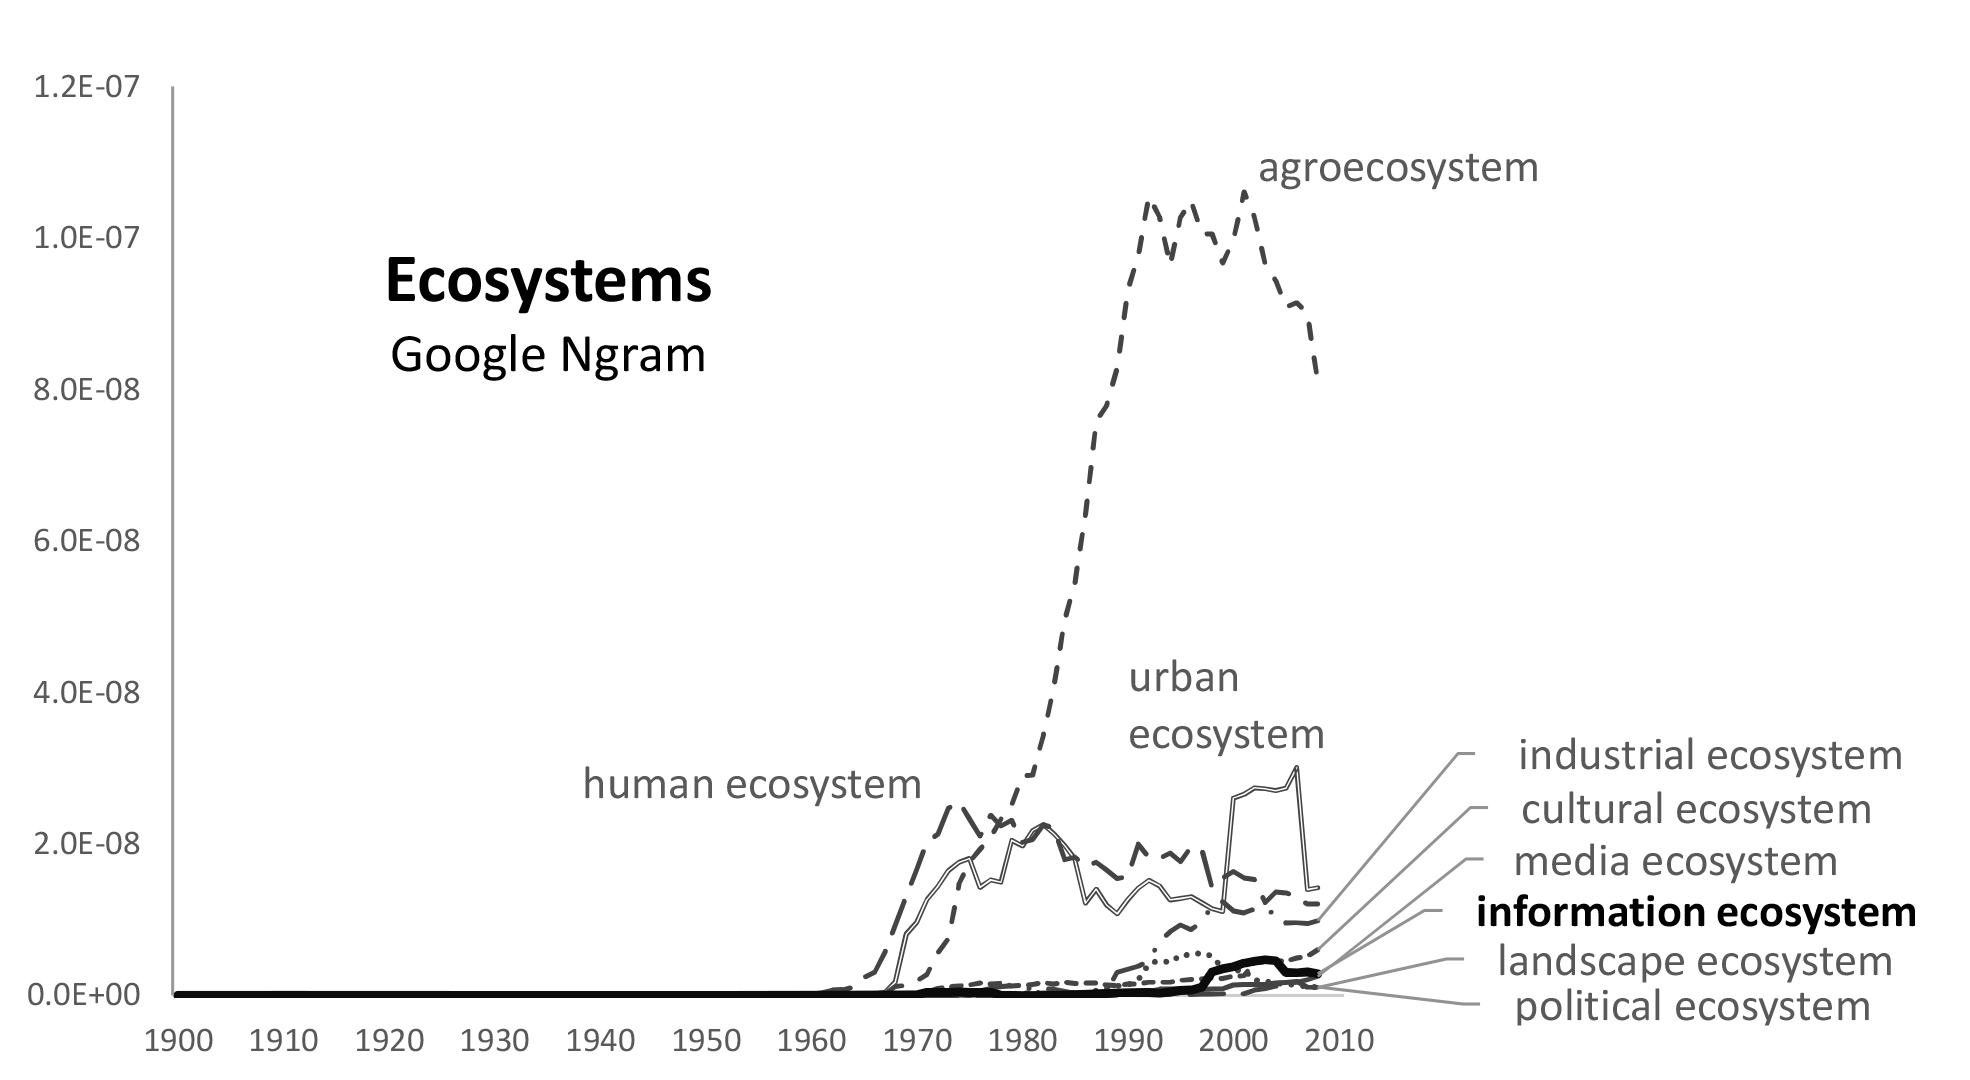
\includegraphics[width=5.5in]{figures/ecosystemsAll}
  \caption{Emergent use varying ecosystem metaphors as a Google Ngram. Compare to figure 2! The use of various ecologies vs various ecosystem metaphors is an order of magnitude higher. It is more common to say information ecology (as a study of information systems using ecological concepts) than it is to say information ecosystem (implying a metaphorical relationship). Note that agro ecology is an exception. While some might say this is a human made ecosystem, it is perhaps more correct to think of it as a human \textit{influenced} ecosystem.}
\end{figure}

Within the academy information ecology is an ecological approach to answering research questions. This might mean using some tools from the ecology toolkit or even thinking broadly about the function of information in mediating relationships between the living and the non-living. On the other hand, an information ecology in the business management literature is the connectedness, the inter-relatedness, the actual set of relationships between human actors, machines and the information itself. It could even refer to the social environment or human community in which information is flowing. In the business management literature an information ecology is almost synonymous with an information ecosystem, yet it rarely has a connection to the natural environment.


\subsection{Big Data as Information Pollution}

As our ability increases to capture more quantities of data does the quality decline? As Niel Postman suggests, "We have transformed information [and data] into a form of garbage" \citep[cited in][p. 50]{stepp_1999}. Does this potential decline in quality information somehow hamper effective decision making or are we able to filter and analyze the data in ways that provide novel insights that improve effective decision making? Or as Barend Mons put it recently, "Data is like oil. We pump it from the earth. We spill it everywhere. We make a mess." \citep{mons_2016}


\subsection{Disappearing Nature}

Our admittedly incomplete review of the literature suggests that the use of the term information ecosystem, either as a metaphor or as a simple vernacular reference, actually renders nature more invisible instead of more visible. Within the three ecology research programs outlined above (cognitive, media, and political), this may not be the case as there are explicit connections to nature and the environment. Yet within the uses of the information ecosystem metaphor--or information ecology metaphor in the sense of relationships, not programs of inquiry--this explicit connection is lacking. Indeed, by claiming that the information system is an ecology (as a set of relations like in an ecosystem) the natural ecosystem becomes invisible. The very real need in an information system for natural resources such as energy, metal and petroleum, and space itself fade into the background of the conversation. It is possible that the use of the term "information ecosystem" or "information ecology" (as the relations) further disconnects us from our natural environment.  As observed in a review of environmental history and environmental studies, this disconnection may indeed be the most pressing problem that human society currently faces. Urgent environmental problems such as climate change and biodiversity loss are only made worse when they are rendered invisible to society \citep{worthy_2013}.
